\documentclass[11pt]{article}
\usepackage[margin=1.15in]{geometry}
\usepackage{amsmath,amssymb,amsthm}
\usepackage{booktabs}
\usepackage{graphicx}
\usepackage{microtype}
\usepackage[authoryear,round]{natbib}
\usepackage[colorlinks=true,linkcolor=black,citecolor=black,urlcolor=black]{hyperref}
\usepackage{setspace}
\onehalfspacing

\newtheorem{proposition}{Proposition}
\theoremstyle{definition}
\newtheorem{definition}{Definition}
\newcommand{\E}{\mathbb{E}}
\newcommand{\Var}{\operatorname{Var}}
\newcommand{\Cov}{\operatorname{Cov}}

\title{What a Correlation of 0.18 Carries\\[4pt]
\large Pooled Cohorts and the Step From a Culture Experiment to a Population Pattern}
\author{Flyxion\\Independent Researcher}
\date{October 2026}

\begin{document}
\maketitle

\begin{abstract}
\noindent
A recent study of gut bacteria combines a series of controlled culture experiments, in which a Gram-negative family promotes a dominant member of another family in the presence of plant polysaccharides, with an analysis of public metagenomes in which a rank correlation of $0.18$ between the two groups appears in non-industrialized populations and is absent in industrialized ones. The culture experiments are well controlled and include knockout strains, multiple isolates, absolute-abundance checks and complex human and mouse communities. The population correlation is a different kind of evidence, and its meaning depends on how the individuals were pooled. This essay shows that a pooled rank correlation of the reported size can arise entirely from differences between cohorts in the two quantities, with no association within any cohort; that the reported $P$ value treats several hundred individuals from a handful of countries as independent, which with a few cohorts and a modest cohort share of variance gives false-positive rates of $8\%$ to $44\%$ for a nominal $5\%$ test under the complete null; and that, by reconstruction from the reported values, a correlation of $0.18$ accounts for about $3\%$ of rank variance. None of this weakens the culture results. It places the population analysis as supporting context and identifies the within-cohort analysis that would let it carry more.
\end{abstract}

\section{Two kinds of evidence in one paper}

The study \citep{tawk2026} asks why some healthy human gut microbiota are dominated by one family of Bacteroidota (Bacteroidaceae) and others by another (Prevotellaceae, represented by \emph{Segatella copri}), a pattern that diet alone does not explain. Its experimental core is a set of synthetic communities passaged in rich medium with 94 dietary components. \emph{S. copri} expands when particular polysaccharides, such as arabinan, are supplied, and the expansion depends on the presence of Enterobacteriaceae, most thoroughly \emph{Escherichia coli}. The authors support this with transcriptomics of the relevant polysaccharide utilization loci, a deletion mutant of \emph{S. copri} that cannot use arabinan, an \emph{E. coli} mutant that cannot metabolize the arabinan-derived sugars but still promotes \emph{S. copri}, multiple \emph{E. coli} and \emph{Segatella} isolates, stabilized human faecal communities and mouse caecal communities. They also address a standard problem with relative-abundance data: the text reports that most supplements did not change the final optical density or total cell number, and quantitative PCR is used for the key organisms.

A last section asks whether the pattern is visible in populations. It analyses $870$ public shotgun metagenomes from healthy adults in $9$ countries, classified as industrialized or non-industrialized. Both \emph{S. copri} and Enterobacteriaceae are more prevalent and more abundant in the non-industrialized group, and within that group the abstract's statement is that there is ``a positive correlation between Segatella-rich non-industrialized microbiomes and Enterobacteriaceae abundance.'' The supporting statistic given in the text is a Spearman correlation between the relative abundance of \emph{S. copri} and the number of Enterobacteriaceae species, $R=0.18$ ($P=0.00045$) in non-industrialized individuals and $R=-0.061$ ($P=0.18$) in industrialized ones.

This essay concerns only that last step. The culture experiments carry the paper's causal weight, and the authors note that the interaction in industrialized microbiomes remains ambiguous. The question is what the population correlation adds.

\section{What the reported numbers imply}

The sample sizes are not stated alongside the correlations in the text read, but they can be recovered from the correlations and their $P$ values using the exact $t$ distribution for a correlation coefficient. This gives $n\approx376$ for the non-industrialized group and $n\approx485$ for the industrialized group, a total of $861$, close to the $870$ metagenomes reported, which supports the reconstruction. Three consequences follow.

First, $R=0.18$ corresponds to $R^2\approx0.032$: about three per cent of the rank variance of one quantity is associated with the other. It is a detectable association and a weak one.

Second, the difference between the two correlations is itself significant under independence. Fisher's transformation gives $z=(\operatorname{arctanh}0.18-\operatorname{arctanh}(-0.061))/\sqrt{1/373+1/482}=3.52$, $P\approx0.0004$. The comparison avoids the error of treating ``significant in one group, not in the other'' as a difference \citep{gelmanstern2006}, and the paper's claim that the groups differ survives that test. It survives it only under the assumption of independent individuals.

Third, the quantity correlated is a relative abundance on one side and a species count on the other. A species count depends on sequencing depth and on the detection threshold (the analysis retains species at relative abundance $\ge10^{-4}$), so a correlation with it mixes biology with detectability.

\section{Pooled correlation can come entirely from between-cohort differences}

Public metagenomes come from studies. Cohorts differ in population, diet, sample handling, sequencing depth and profiling choices, and the two quantities can differ in mean from cohort to cohort for reasons unrelated to any interaction between the organisms. Suppose there are $K$ cohorts. Let the two standardized quantities be $x=\mu_c+\epsilon$ and $y=\nu_c+\eta$, where $(\mu_c,\nu_c)$ are cohort effects, $\epsilon,\eta$ are independent within-cohort noise, and the within-cohort correlation is zero.

\begin{proposition}
Let the share of the variance of $x$ and of $y$ due to cohort be $s_x$ and $s_y$, and let the correlation between the cohort effects be $\rho_b$. If the within-cohort correlation is zero, the pooled Pearson correlation is $\rho_b\sqrt{s_xs_y}$.
\end{proposition}

\begin{proof}
The pooled covariance is $\Cov(\mu_c,\nu_c)=\rho_b\sqrt{s_xs_y}$ for unit-variance variables, since the within-cohort terms are uncorrelated.
\end{proof}

With $s_x=s_y=0.3$ and $\rho_b=0.6$, which asks only that the cohorts with more \emph{S. copri} are, on average, those with more Enterobacteriaceae species, the pooled correlation is $0.18$, the reported value. It requires no association within any cohort. Table~\ref{tab:pooled} gives simulated pooled Spearman correlations for $N=374$ individuals in $K$ cohorts and the rejection rate of the naive test, which treats all individuals as independent.

\begin{table}[h]
\centering
\caption{Simulated pooled Spearman correlation, with zero association within every cohort, and rejection rate of the naive test at nominal $0.05$ (3000 replicates, $N=374$). $s$ is the cohort share of variance in each variable and $\rho_b$ the correlation between cohort effects.}
\label{tab:pooled}
\small
\begin{tabular}{rrrccc}
\toprule
$K$ & $s$ & $\rho_b$ & mean pooled $R$ & sd of $R$ & naive rejection rate \\
\midrule
4 & 0.1 & 0.0 & $-0.001$ & 0.065 & 0.121 \\
4 & 0.1 & 0.6 & 0.043 & 0.069 & 0.199 \\
4 & 0.3 & 0.0 & $0.000$ & 0.134 & 0.438 \\
4 & 0.3 & 0.6 & 0.121 & 0.135 & 0.544 \\
9 & 0.1 & 0.0 & 0.001 & 0.059 & 0.080 \\
9 & 0.1 & 0.6 & 0.050 & 0.060 & 0.203 \\
9 & 0.3 & 0.0 & 0.003 & 0.103 & 0.324 \\
9 & 0.3 & 0.6 & 0.152 & 0.103 & 0.680 \\
\bottomrule
\end{tabular}
\end{table}

The second point of the table is the rate of false positives. With $\rho_b=0$, the cohort effects are independent and there is no association of any kind, yet the naive test rejects in $8\%$ to $44\%$ of replicates, depending on the number of cohorts and their share of variance. The reason is that the effective sample size for the between-cohort part of the correlation is the number of cohorts, not the number of individuals. A correlation among $K=4$ cohort means is a correlation among four points, and individuals within cohorts do not add independent information about it. The naive $P=0.00045$ for $n=376$ would then describe the precision of a quantity that is dominated by a handful of cohort positions.

\begin{figure}[h]
\centering
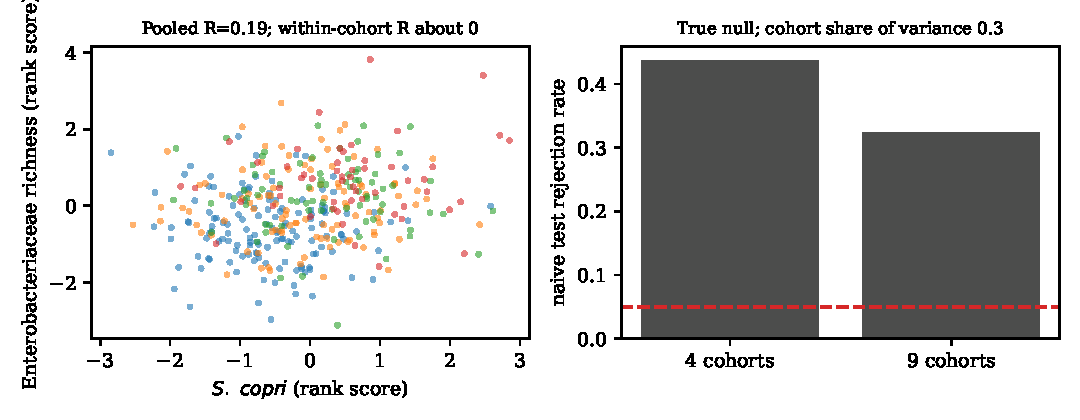
\includegraphics[width=\textwidth]{fig_pooled.pdf}
\caption{Left: simulated individuals from four cohorts, with no association within any cohort (within-cohort rank correlations between $-0.05$ and $0.04$), pooled rank correlation $0.19$. Right: rejection rate of the naive test when there is no association of any kind and cohorts account for $30\%$ of the variance of each variable.}
\label{fig:pooled}
\end{figure}

\section{What is and is not known about the actual data}

The portions of the paper read here do not state the number of cohorts in each lifestyle category or the share of variance due to cohort, so the simulation is a statement about what is possible and not about what happened. Both quantities plausibly differ by cohort: the paper itself reports that \emph{S. copri} and Enterobacteriaceae are each more prevalent in some populations than others, which is the kind of structure that makes $\rho_b$ positive. Profiling choices and depth, which differ by study, bear on the species-count variable. Whether the within-category correlation survives conditioning on cohort is therefore the open empirical question, and it is the one on which the population evidence for the interaction depends.

The group-level pattern, that both organisms are enriched in non-industrialized populations, is different again. It is expected under many hypotheses, including a shared cause such as diet or environmental exposure, and does not discriminate the proposed interaction from them. A difference in prevalence between populations is a statement about populations, and the interaction concerns what happens within a gut.

\section{A note on the word synergy}

Within the culture experiments, the reported statements take the form that supplementation promotes \emph{S. copri} when \emph{E. coli} is present but not when it is absent, with significance judged by pairwise comparisons corrected for multiple testing, on three biological replicates per condition. A synergy or dependence of this kind is an interaction: the effect of supplementation differs between the two \emph{E. coli} conditions. The direct statistic for that is the contrast of differences, with its own interval, and not two separate comparisons, one significant and one not. The earlier essay on paired inference states the underlying point, that the difference between significant and not significant is not itself a significant difference \citep{gelmanstern2006}. Here the quantities are large in the figures described and the contrast is likely to be clear, so the issue is one of reporting, but with $n=3$ and a bounded outcome, an interval on the interaction contrast, ideally on the scale of the log ratio of \emph{S. copri} to Bacteroidaceae that the paper uses elsewhere, is the appropriate summary.

\section{What would let the population analysis carry more}

\begin{enumerate}
\item Report the correlation within each cohort, and combine them in a random-effects meta-analysis, so that the unit of replication is the cohort.
\item Report the number of cohorts per lifestyle category and the cohort share of variance in each variable.
\item Use a permutation test that shuffles within cohort, or a mixed model with a cohort effect, so that between-cohort covariation cannot generate the result.
\item Adjust for sequencing depth, and replace the species count by a measure that does not depend on it, such as presence above a fixed read-count threshold or a rarefied richness.
\item Compare the two lifestyle categories with a test for the difference of correlations that accounts for clustering.
\end{enumerate}
If the within-cohort correlation remains positive and similar in several cohorts, the population evidence becomes an independent confirmation, since it comes from a setting where the experimenters' conditions did not apply.

\section{Conclusion}

The culture experiments establish, with controls the paper describes, that the presence of a Gram-negative bacterium and a plant polysaccharide together favour \emph{S. copri} over Bacteroidaceae in the communities tested. The population correlation of $0.18$ is evidence of a different grade. Pooled over countries, a coefficient of this size can arise from cohort differences alone, and the nominal $P$ value measures the wrong sample size. The accurate role of that analysis is to show that the organisms co-occur at the population level, which is what a shared cause would also produce. The within-cohort analysis would show more.

\begin{thebibliography}{9}
\bibitem[Gelman and Stern(2006)]{gelmanstern2006} Gelman, A., Stern, H. (2006). The difference between ``significant'' and ``not significant'' is not itself statistically significant. \emph{The American Statistician} 60(4), 328--331.
\bibitem[Tawk et al.(2026)]{tawk2026} Tawk, C., El Mouali, Y., Huang, K.~D., Valkiers, S., Heidrich, V., Gronow, A., Osbelt, L., Rapp, J., Link, H., Segata, N., Typas, A., Strowig, T. (2026). Synergy between Enterobacteriaceae and diet mediates competition between dominant Bacteroidales in the human gut. \emph{Nature Microbiology}. doi:10.1038/s41564-026-02500-6.
\end{thebibliography}

\end{document}
